\documentclass{exam}
\usepackage{../../commonheader}
\usepackage{graphicx}
\usepackage{color}

%%% CHANGE THESE %%%%%%%%%%%%%%%%%%%%%%%%%%%%%%%%%%%%%%%%%%%%%%%%%%%%%%%%%%%%%%
\discnumber{3}
\title{\textsc{Final Review}}
\date{May 3, 2017}
%%%%%%%%%%%%%%%%%%%%%%%%%%%%%%%%%%%%%%%%%%%%%%%%%%%%%%%%%%%%%%%%%%%%%%%%%%%%%%%

\begin{document}
\maketitle
\rule{\textwidth}{0.15em}
\fontsize{12}{15}\selectfont

%%% INCLUDE TOPICS HERE %%%%%%%%%%%%%%%%%%%%%%%%%%%%%%%%%%%%%%%%%%%%%%%%%%%%%%%


%%% Question %%%

\section{Binary Trees}
\begin{questions}

\item Given a binary tree \texttt{t}, determine whether or not it is a valid Binary Tree.
\newline
\begin{lstlisting}
def valid_bst(t):

  def helper(t, minVal, maxVal):

    if ____________________:

      return True 

    check_left = ________________________________

    check_right = _______________________________

    if ___________________________________: 

      if check_left and check_right:

        return True

    return False

  return _____________________________________
\end{lstlisting}
\begin{solution}
\begin{lstlisting}
Given a binary tree t, determine whether or not it is a valid BST 
def valid_bst(t):
  def helper(t, minVal, maxVal):
    if t is BinTree.empty:
      return True 
    check_left = helper(t.left, minVal, t.label)
    check_right = helper(t.right, t.label, maxVal)
    if t.label >= minVal and t.label <= maxVal:
      if check_left and check_right:
        return True
    return False
  return helper(t, -float('inf'), float('inf'))
\end{lstlisting}
\end{solution}

\clearpage

\item Given a Binary Tree, \texttt{t} and an integer \texttt{k}, return the sum of all entries 
in the Binary Tree at or within 1 level of the \texttt{k}th level. The root is at level 0. You may assume that all entries are integers. Let the \texttt{t} in the doctests be the following tree:
\begin{center}
 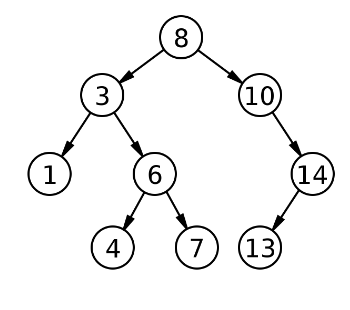
\includegraphics[scale=0.7]{approxLevelSum}
\end{center}

\begin{lstlisting}
def approxLevelSum(t, k):
  """
  >>> approxLevelSum(t, 1)
  42  #8 + 3 + 10 + 1 + 6 + 14 
  >>> approxLevelSum(t, 2)
  58 
  >>> approxLevelSum(t, 3)
  45
  >>> approxLevelSum(t, 0)
  21
  """
  if ____________________________________:

      return 0

  elif ____________________________________:

      return t.label

  elif ____________________________________:

      return ________________________________________________

  else:

      return ________________________________________________
\end{lstlisting}

\begin{solution}
\begin{lstlisting}
def approxLevelSum(t, k):
    if t is BinTree.empty:
        return 0
    elif k == -1:
        return t.label
    elif k <= 1:
        return approxLevelSum(t.left, k - 1) + 
approxLevelSum(t.right, k - 1) + t.label
    else:
        return approxLevelSum(t.left, k - 1) + 
approxLevelSum(t.right, k - 1)
\end{lstlisting}
\end{solution}
\end{questions}
\clearpage

% ################################################################
% ################################################################
% ################################################################

\section{Sets}
\begin{questions}

\item Given a list of lists of letters, write a solution that will return a list of the letters in every single list in the input. You may assume that the input list contains at least one list.
\newline
\begin{lstlisting}
def common_letters(letterLists):
  """
  >>> one, two = ['a', 'b', 'c'], ['d', 'c', 'b']
  >>> three = ['c', 'e']
  >>> common_letters([one, two, three])
  ['c']
  """
  result = __________________________________________

  for _______________________________________________________:

    result = _______________________________________________

  return __________________________________________
\end{lstlisting}
\begin{solution}
\begin{lstlisting}
def common_letters(letterLists):
    result = set(letterLists[0])
    for lst in letterLists[1:]:
      result = result.intersect(set(lst))
    return list(result)
\end{lstlisting}
\end{solution}
\end{questions}


% ################################################################
% ################################################################
% ################################################################

\section{Streams}
\begin{questions}
\item Let's say we were to modify the rest function in the stream class
\begin{lstlisting}
@property 
def rest(self):
  if self._compute rest is not None: 
    print(“computing rest”)
    self._rest = self._compute rest() 
    self._compute rest = None 
  return self._rest
\end{lstlisting}

What would Python display if we executed the following code?
\begin{center}
    \begin{tabular}{|m{9.2cm}|m{6cm}|}
\hline
\textbf{Expression} & \textbf{Interactive Output} \\
\hline
\lstinline$>>> int_strm = make_integer_stream()$
 \lstinline$>>> print(int_strm.rest)$ & \\
 & \\ & \\
\hline
\lstinline$>>> print(int_strm.rest)$ & \\ & \\
\hline
\end{tabular}
\end{center}

\begin{solution}
\begin{center}
    \begin{tabular}{|m{9cm}|m{6cm}|}
\hline
\textbf{Expression} & \textbf{Interactive Output} \\
\hline
\lstinline$>>> int_strm = make_integer_stream()$
 \lstinline$>>> print(int_strm.rest)$ & \color{red}\lstinline$computing rest$ \\
 & \color{red}\lstinline$Stream(2, <...>)$ \\ & \\
\hline
\lstinline$>>> print(int_strm.rest)$ & \color{red}\lstinline$Stream(2, <...>)$ \\ & \\ & \\
\hline
\end{tabular}
\end{center}
\end{solution}

\item Takes in a list, \texttt{lst} and a positive integer \texttt{i} and returns an infinite stream of every \texttt{i}th element in \texttt{lst}. If the \texttt{lst} has no more elements, cycle back to the beginning of \texttt{lst} and continue counting. 
\begin{lstlisting}
def cycle_ith(lst, i):
  seen = 0

  while seen < i:

    curr = ___________

    __________________

    lst.append(curr)

    __________________

  ______________________________________
\end{lstlisting}
\begin{solution}
\begin{lstlisting}
def cycle_ith(lst, i):
  seen = 0
  while seen < i:
    curr = lst[0]
    lst = lst[1:]
    lst.append(curr)
    seen += 1
  return Stream(curr, lambda: cycle_ith(lst, i))
\end{lstlisting}
\end{solution}

\item Takes in a stream and returns a new stream that contains each element of the input stream only once and in the same order. This function should work for both finite and infinite streams.
\newline
\begin{lstlisting}
def set_stream(s):
  seen = []

  def compute_rest(curr_stream):

    if _____________________________:

      ______________________________

    if _____________________________:

      seen.append(curr_stream.first)

      _______________________________________

    else:

      _______________________________________
  return compute_rest(s)
\end{lstlisting}
\begin{solution}
\begin{lstlisting}
def set_stream(s):
  seen = []
  def compute_rest(curr_stream):
    if curr_stream is Stream.empty:
      return Stream.empty
    if curr_stream.first not in seen:
      seen.append(curr_stream.first)
      return Stream(curr_stream.first, lambda:compute_rest(curr_stream.rest))
    else:
      return compute_rest(curr_stream.rest)
  return compute_rest(s)
\end{lstlisting}
\end{solution}
\end{questions}

% ################################################################
% ################################################################
% ################################################################

\section{Scheme}
\begin{questions}

\item What Would Scheme Display?
\begin{center}
    \begin{tabular}{|m{9cm}|m{6cm}|}
\hline
\textbf{Expression} & \textbf{Interactive Output} \\
\hline
\lstinline$scm> 'csm$ & \\ & \\ & \\
\hline
\lstinline$scm> (if 0 1 (/ 1 0))$ & \\ & \\ & \\
\hline
\lstinline$scm> (or 1 and 2)$ & \\ & \\ & \\
\hline
\lstinline$scm> (and 1 2)$ & \\ & \\ & \\
\hline
\lstinline$scm> (or 1 2)$ & \\ & \\ & \\
\hline
\lstinline$scm> (/ 5)$ & \\ & \\ & \\
\hline
\lstinline$scm> (* 5)$ & \\ & \\ & \\
\hline
\lstinline$scm> (- 5)$ & \\ & \\ & \\
\hline
\lstinline$scm> (+ 5)$ & \\ & \\ & \\
\hline
\end{tabular}
\end{center}

\begin{solution}
% TODO FILL OUT THIS SOLUTION
\begin{center}
    \begin{tabular}{|m{9cm}|m{6cm}|}
\hline
\textbf{Expression} & \textbf{Interactive Output} \\
\hline
\lstinline$>>>int_strm = make_integer_stream()$
 \lstinline$>>>print(int_strm.rest)$ & \color{red}\lstinline$computing rest$ \\
 & \color{red}\lstinline$Stream(2, <...>)$ \\ & \\
\hline
\lstinline$>>>print(int_strm.rest)$ & \color{red}\lstinline$Stream(2, <...>)$ \\ & \\ & \\
\hline
\end{tabular}
\end{center}
\end{solution}

\item Draw the box and pointer diagrams for the following lists.

\begin{tabular}{m{7cm} m{6cm}}
\begin{lstlisting}
scm> '(1 2 3)
\end{lstlisting}
\begin{solution}
\begin{center}
 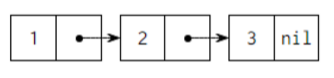
\includegraphics[scale=0.7]{bp1}
\end{center}
\end{solution}
&
\begin{lstlisting}
scm> '(1 (2 (3 (4))))
\end{lstlisting}
\begin{solution}
\begin{center}
 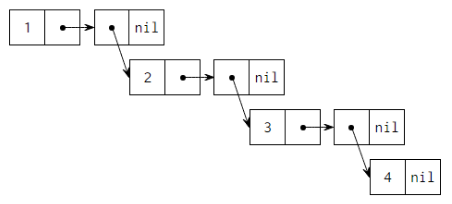
\includegraphics[scale=0.7]{bp2}
\end{center}
\end{solution}
\end{tabular}
\end{questions}
% ################################################################
% ################################################################
% ################################################################

\section{Interpreters}
\begin{center}
 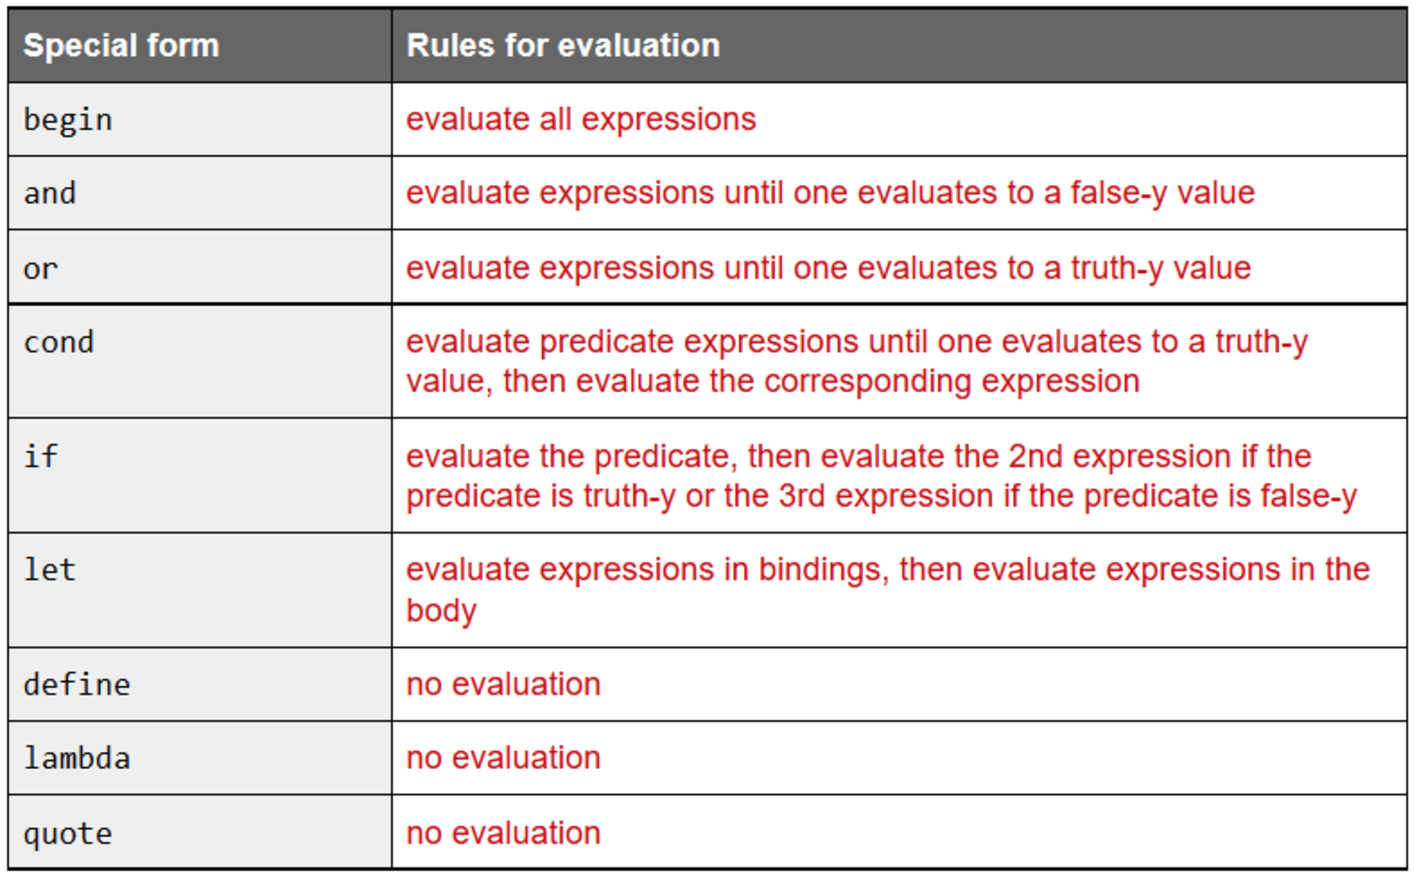
\includegraphics[scale=0.6]{evalRules}
\end{center}
\begin{questions}
\item How many calls to \texttt{scheme\_eval}? How many calls to \texttt{scheme\_apply}?
\begin{center}
    \begin{tabular}{|m{12cm}|m{1.5cm}|m{1.5cm}|}
\hline
\textbf{Expression} & \textbf{Eval} & \textbf{Apply} \\
\hline
\lstinline$(and 'pizza 'with 'pepperoni #f 'pineapple)$ &  & \\ & & \\ & &  \\
\hline
\lstinline$(lambda (cs61a) cs61a)$ & & \\ & & \\ & & \\
\hline
\lstinline$(if 6 1 (+ 1 0))$ & &\\ & & \\ & & \\
\hline
\lstinline$(define (gibbesify g) $ & & \\
\lstinline$   (cond  $ & & \\
\lstinline$      ((= g 0) 'schemineverday)$ & & \\
\lstinline$      ((= g 1) (gibbesify (- g 1))$ & & \\
\lstinline$      (else (gibbesify (- g 2)))$ & & \\
\hline
\lstinline$(let ((condvoluted gibbesify)) (condvoluted 2))$ & &\\ & & \\ & & \\
\hline
\end{tabular}
\end{center}

\begin{solution}
\begin{center}
    \begin{tabular}{|m{12cm}|m{1.5cm}|m{1.5cm}|}
\hline
\textbf{Expression} & \textbf{Eval} & \textbf{Apply} \\
\hline
\lstinline$(and 'pizza 'with 'pepperoni #f 'pineapple)$ & {\color{red}5} & {\color{red}0} \\ & & \\ & &  \\
\hline
\lstinline$(lambda (cs61a) cs61a)$ & {\color{red}1} &  {\color{red}0} \\ & & \\ & & \\
\hline
\lstinline$(if 6 1 (+ 1 0))$ & {\color{red}3} & {\color{red}0} \\ & & \\ & & \\
\hline
\lstinline$(define (gibbesify g) $ & {\color{red}1} & {\color{red}0} \\
\lstinline$   (cond  $ & & \\
\lstinline$      ((= g 0) 'schemineverday)$ & & \\
\lstinline$      ((= g 1) (gibbesify (- g 1))$ & & \\
\lstinline$      (else (gibbesify (- g 2)))$ & & \\
\hline
\lstinline$(let ((condvoluted gibbesify)) (condvoluted 2))$ & {\color{red}26} & {\color{red}6}\\ & & \\ & & \\
\hline
\end{tabular}
\end{center}
\end{solution}
\end{questions}


% ################################################################
% ################################################################
% ################################################################

\section{Tail Recursion}
\begin{questions}

\item Is it tail recursive?
\begin{center}
    \begin{tabular}{|m{13cm}|m{1.5cm}|}
\hline
\textbf{Expression} & \textbf{Yes/No} \\
\hline
\lstinline$(define (cream cheese)$ &  \\
\lstinline$    (if (null? cheese)$ & \\ 
\lstinline$        0$ & \\
\lstinline$        (+ (car cheese) (cream (cdr cheese)))))$ & \\
\hline
\lstinline$(define (introducing professor dog)$ &  \\
\lstinline$    (if (null? professor)$ & \\ 
\lstinline$        dog$ & \\
\lstinline$        (introducing (cdr professor) (+ (car professor) dog))))$ & \\
\hline
\lstinline$(define (fact n)$ &  \\
\lstinline$    (if (= n 1)$ & \\ 
\lstinline$        n$ & \\
\lstinline$        (* n (fact (- n 1)))))$ & \\
\hline
\end{tabular}
\end{center}

\item Here are constructors and selectors for a Binary Tree.

\begin{tabular}{m{9cm} m{7cm}}
\begin{lstlisting}
(define (tree entry left right)
  (cons entry (cons left right)))

(define (entry tree)
  (car tree))
  \end{lstlisting} & 
\begin{lstlisting}
(define (left tree)
  (car (cdr tree)))

(define (right tree)
  (cdr (cdr tree)))
  \end{lstlisting}

\end{tabular}

This procedure takes a binary search tree, as well as an item contained in the binary search tree. It returns a list of the values encountered along the path from the root to the node containing that item. The \texttt{t} in the doctests is defined as follows:
\begin{center}
 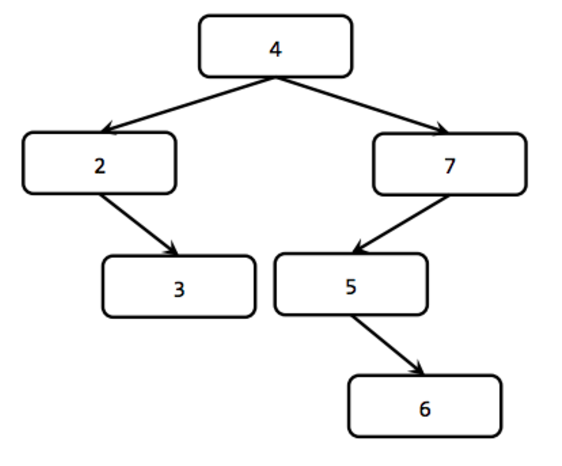
\includegraphics[scale=0.7]{bstPath}
\end{center}


\clearpage

\begin{lstlisting}[language=Scheme]
(define (bst-path bst item)
\end{lstlisting}

\begin{solution}[6cm]
\begin{lstlisting}
(define (bst-path bst item) 
  (define (bst-helper tree item acc)
    (cond ((= (entry tree) item) (append acc (list item)))
      ((> (entry tree) item) 
        (bst-helper (left tree) item (append acc (list (entry tree))))) 
      (else (bst-helper (right tree) item (append acc (list (entry tree)))) )
    )
  ) 
(bst-helper bst item nil))
\end{lstlisting}
\end{solution}
\end{questions}

% ################################################################
% ################################################################
% ################################################################

\section{SQL}
\begin{questions}

\item We can use SQL to determine the anagrams of a word! Specifically, let’s use SQL to find the anagrams of 'paul'.

\begin{lstlisting}[language=SQL]

        with
          given (char, weight) as (
            select 'p' , 0001 union
            select 'a' , 0010 union
            select 'u' , 0100 union
            select 'l' , 1000
          )

        select _______________________________ 

        ______________________________________

        from _________________________________ 

        ______________________________________ 

        where ________________________________;

\end{lstlisting}

\begin{solution}
\begin{lstlisting}[language=SQL]
with
  given (char, weight) as (
    select 'p' , 0001 union
    select 'a' , 0010 union
    select 'u' , 0100 union
    select 'l' , 1000
  )

select a.char || b.char || c.char || d.char 
from given as a, given as b, given as c, given as d 
where a.weight + b.weight + c.weight + d.weight = 1111;
\end{lstlisting}
\end{solution}

\clearpage

\item After more than 100 years of operation, the Ringling Bros. circus is closing.  A victory for animal rights advocates, the circus’ closure poses a challenge for the zoologists tasked with moving the circus’ animals to more suitable habitats.
 
The zoologists must first take the animals in a freight elevator with a weight limit of 2000.  In order to speed-up the process, the zoologists prefer to take groups of animals of the same species in the elevator, rather than one animal at a time.  

Assume the zoologists will only put all of the animals of a particular species in the elevator, or take animals of that particular species one at a time.

You have access to the table \texttt{animals}, with columns containing the animals’ names, weights, and species.

Write a query that returns the collective weight and species of animals in a group where there is more than one animal of a particular species in a group, and the collective weight of the animals in the group is less than 2000.

Your query should yield the following result:

\begin{lstlisting}[language=SQL]
229 pig
1618 tiger
91 dog
\end{lstlisting}

\begin{lstlisting}[language=SQL]

    select _____________________________ 

    from __________________________

    group by _______________________________

    having 
    ______________________________;
    
\end{lstlisting}
\begin{solution}
\begin{lstlisting}[language=SQL]
 
select sum(weight), species
from animals
group by species
having count(*) > 1 and sum(weight) < 2000;
\end{lstlisting}
\end{solution}

\item Now, suppose we have a table height that has the animals' names and heights.  Suppose we want to join the tables animals and height.  How many rows will the joined table have?
\begin{solution}[2cm] 121 \end{solution}

\clearpage

\item To take the animals to their new habitats, the zoologists load the animals into trucks.  The zoologists again want to take the animals in groups of the same species, but one of the trucks has a height limit of 5.0.
 
Write a query that returns the maximum height and species of animals in a group where the maximum height is less than 5.0.  Your query may yield a species where there is only one animal of that particular species.

Your query should yield the following result:
\begin{lstlisting}[language=SQL]
4.1 pig
4 dog
4.9 zebra
\end{lstlisting}

\begin{lstlisting}[language=SQL]

    select _____________________________ 

    from __________________________

    where__________________________

    group by _______________________________

    having 
    ______________________________;
\end{lstlisting}

\begin{solution}
\begin{lstlisting}[language=SQL]
 
select max(height), species
from animals as a, 
height as b
where a.name = b.name
group by species
having max(height) < 5.0;
\end{lstlisting}
\end{solution}

\end{questions}

%%%%%%%%%%%%%%%%%%%%%%%%%%%%%%%%%%%%%%%%%%%%%%%%%%%%%%%%%%%%%%%%%%%%%%%%%%%%%%%

\end{document}
